% This is samplepaper.tex, a sample chapter demonstrating the
% LLNCS macro package for Springer Computer Science proceedings;
% Version 2.20 of 2018/03/10
%
\documentclass[runningheads]{llncs}
\usepackage{graphicx}%
\usepackage{multirow}%
\usepackage{amsmath,amssymb,amsfonts}%
\usepackage{amsthm}%
\usepackage{mathrsfs}%
\usepackage[title]{appendix}%
\usepackage{xcolor}%
\usepackage{textcomp}%
\usepackage{manyfoot}%
\usepackage{booktabs}%
\usepackage{algorithm}%
\usepackage{algorithmicx}%
\usepackage{algpseudocode}%
\usepackage{listings}%
\usepackage[T1]{fontenc}
\def\doi#1{\href{https://doi.org/\detokenize{#1}}{\url{https://doi.org/\detokenize{#1}}}}
%
\usepackage{graphicx}
% Used for displaying a sample figure. If possible, figure files should
% be included in EPS format.
%
% If you use the hyperref package, please uncomment the following line
% to display URLs in blue roman font according to Springer's eBook style:
% \renewcommand\UrlFont{\color{blue}\rmfamily}
%
\usepackage{listings}
\lstset{language=Pascal}
% Please use the

\begin{document}
%
\title{Reactive Maintenance Scheduling\thanks{Supported by organization x.}}
%
%\titlerunning{Abbreviated paper title}
% If the paper title is too long for the running head, you can set
% an abbreviated paper title here
%
\author{Christian Brunbjerg Jespersen\inst{1}\orcidID{0000-1111-2222-3333}}
%
\authorrunning{C. Jespersen et al.}
% First names are abbreviated in the running head.
% If there are more than two authors, 'et al.' is used.
%
\institute{Technical University of Denmark, Kongens Lyngby 2800, Denmark 
\email{cbrje@dtu.dk}\\
}
%
\maketitle              % typeset the header of the contribution
%
\begin{abstract}
The abstract should briefly summarize the contents of the paper in
150--250 words.

\keywords{Hierarchical Models  \and Reactive Scheduling \and Actor based Large Neighborhood Search}
\end{abstract}
%
%
%
\section{Reactive Maintenance Scheduling}
Maintenance scheduling is by its nature an uncertain process, breakdowns are difficult to predict and due to the often critical nature of corrective maintenance resources (technicians) often have to be ready to repair the underlying equipment. Traditionally maintenance is scheduled as a resource constrained project scheduling problem (RCPSP), that inherently has some level of aggregation build in to handle the uncertainty. 

In the literature there have been developed different theories and principles to make the RCPSP able to handle increasing levels of uncertainty. These include but are not limited to:

\begin{itemize}
    \item Stochastic optimization
    \item Fuzzy logic
    \item Robust optimization
\end{itemize}

There are multiple hidden assumptions behind the use of these approaches and this paper will argue that to handle the uncertainty present in maintenance scheduling a different approach is needed. First, \textbf{stochastic optimization} is often impractical to apply due to the singular nature of many maintenance tasks, meaning that acquiring the amount of data needed to perform the scenario generation is challenging. Second, \textbf{fuzzy logic} is actually a good approach and is a concept that could be applicable to maintenance optimization but is not considered in this paper. This is primarily due to maintenance being scheduled so technicians and team leaders get a pool of jobs to select from, so that they can adjust the schedule daily during execution, this real-time shuffling makes something like fuzzy logic ineffective as the days that are assigned for each project can move around continuously. To overcome this issue you would have to enforce the statically generated schedule which will be daunting challenging in practice. Third, \textbf{robust optimization} robust can be seen as a more practical implementation of the stochastic optimization, where instead of optimizing the schedule over a set of scenarios you instead include buffers on the jobs and activities. Robust optimization is usually applied in practice where it contributes to one of the main inefficiencies found in maintenance scheduling. Maintenance scheduling is usually focused on availability of the underlying equipment, so a common approach is to schedule in buffers on the resources (technicians) so that you are always ready to respond to a breakdown on critical equipment. 

This paper proposes a different approach based on reactive and interactive models. To achieve these properties, compromises and novelties have to be made and introduced for the scheduling system as a whole to have the desired characteristics. In this paper these compromises and novelties are grouped into the following three subsections: hierarchical model setup, continuous optimization, and user interaction.


\subsection{Hierarchical Model Setup}
In standard maintenance scheduling the process is usually divided up into three distinct processes:
\begin{itemize}
    \item \textbf{A long term strategic schedule}
    \item \textbf{A weekly tactical schedule}
    \item A daily operational schedule
\end{itemize}

Each of these schedules represents a process with distinct objectives and constraints, and this naturally leads to a each schedule having its own model. As uncertainty aggregates as time passes we get into a situation where there is a considerable more uncertainty on the long term strategic perspective than in the two shorter term models. This means that if you were to try and model the long term strategic model using the weekly tactical model, it would be hard to assign meaning to the solution of the model as the variables and constraints model data which we have little ability to reason about. This paper will look at the interplay between the strategic schedule and the tactical schedule leaving the operational schedule for future work. 

\subsubsection{The Strategic Model}
The strategic schedule has three main goals.

\begin{itemize}
    \item prioritization of jobs
    \item levelization of resources
    \item creation of a stable and unique schedule
\end{itemize}

To achieve these goals within the additional requirements of reactivity and interactivity while also being scalable for problem instances containing up to 10000 jobs (~20000 activities). The maintenance scheduling problem
is formulated as a multi-compartment multi-knapsack knapsack problem (MCMKKP). This model has been carefully chosen to give some desirable model characteristics which the RCPSP lacks either directly or indirectly. 
First, getting a stable and unique schedule with 20000 activities in a RCPSP is extremely challenging as the problem is NP-complete with the RCPSP you will have a variable 
for each \textbf{day} and for each \textbf{activity} with corresponding constraints, where for the MCMKKP we only have to variable for each \textbf{peried} and \textbf{job}. This of course simplifies the problem considerably
but it also provides a new characteristic that is crucial for a long term maintenance schedule. This is the property of allowing for gradual reduction in the resource capacity through out the periods. Modifing the RCPSP to get
this property is not trivial as it requires that jobs and activities should be handled differently based of the period they are scheduled in. Besides being difficult it also alters the interpretation of the problem
in an undesirable way by assigning scheduling a job and its activities differently depending on when in the schedule it is placed. Given this justification we will move on to explaining the model itself. 


The first model is the strategic model. The model is comprised of five different sets. Here: P
is the number of periods; O is the number of work
orders; R is the number of resources, Q is a
set which defines the work orders which should
be excluded from a specific period; P is an inclu-
sion set that defines the work orders which should
be included in each period. The model introduces
four different parameters. Here: v_{po}is the value
associated with work order o in period p; $penalty$ paid for exceeding the resource capacity; w_{or} is the capacity needed for work order o
by resource r; c_{pr} amount of capacity
available in period p for resource r. As for the
decision-variables, here: x_{po} is a binary decision-
variable equal to one if work order o is in period
p and zero otherwise; p_{pr} is non-negative decision
variable equal to the amount of excess capacity
above the c_{pr} in period p for resource r.


\begin{alignat}{2}
    &\text{Min} \quad \sum_{p = 1}^{P} \sum_{o = 1}^{O} cost_{po} \cdot x_{po} - \sum_{p = 1}^{P} \sum_{r = 1}^R penalty \cdot excess_{pr} \label{eqn:objective_function_strategic} \\[1em]
    &\text{subject to:} \notag\\[1em]
    &\sum_{o=1}^m w_{or} \cdot x_{po} \leq \ c_{pr} + p_{pr} \quad  && \forall p \in \{1..P\}, \forall r \in \{1..R\}\label{eqn:capacity_constraint} \\[1em]
    &\sum_{p = 1}^{P} x_{po} \leq \ 1 \quad                         && \forall o \in \{1..O\}   \label{eqn:single_workorder_constraint}\\[1em]
    &x_{po} = 0                                                     && \forall (p, o) \in Q \quad  \label{eqn:exclusion_constraint} \\[1em]
    &x_{po} = 1                                                     && \forall (p, o) \in P \quad  \label{eqn:inclusion_constraint}\\[1em]
    &x_{po} \in \{0, 1\}                                            && \forall p \in \{1..P\}, \notag \\
    &&& \forall o \in \{1..O\}                 \label{eqn:x_integrality_constraint}\\[1em] 
    &excess_{pr} \in \mathbb{R}^{+}                                      && \forall p \in \{1..P\}, \notag \\
    &&&\forall r \in \{1..R\}                  \label{eqn:p_non_negativity_constraint}
\end{alignat}

\subsubsection{The Tactical Model}

\begin{alignat}{2} 
& \min && \sum_{o \in O} \omega_o \cdot T_o + \sum_{wc \in WC, d \in D} \lambda \cdot s_{wc,d} \label{eqn:tactical_objective}
\end{alignat}

\begin{alignat}{2}
    &\text{subject to:}\notag \\
    &\sum_{d \in D} x_{k,d} = Q_k \sum_{d \in D} p_{k,d}                                        \ \ && \forall k \in K                              \label{eqn:tactical_complete_work}  \\[1em]
    &x_{k,d} \leq q_k \sum_{\pi} \Pi_{k, \pi, d} \cdot p_{k\pi}                                 \ \ && \forall d \in D, \forall k \in K             \label{eqn:tactical_operating_time} \\[1em]
    &\sum_{\pi} p_{k\tau} = 1                                                                   \ \ && \forall k \in K                              \label{eqn:tactical_one_pattern}    \\[1em]
    &p_{k,d} = 0                                                                                \ \ && \forall k \in K, \forall d < \alpha_k        \label{eqn:tactical_earliest_starting_time} \\[1em]
    &\sum_{d \in D} d \cdot p_{k_1,d}                                                           \ \ && \notag \\
    & = \sum_{d \in D} d \cdot p_{k_2,d}                                                        \ \ && \forall (k_1, k_2) \in \eta                  \label{eqn:tactical_start_start}    \\[1em]
    &\sum_{d \in D} (d + \delta_k) \cdot p_{k_1,d} + \mu_{k_2}                                  \ \ && \notag \\
    & = \sum_{d \in D} d \cdot p_{k_2,d}                                                        \ \ && \forall (k_1, k_2) \in \theta                \label{eqn:tactical_finish_start} \\[1em]
    &\sum_{k} P_k \cdot x_{k,d}                                                                 \ \ && \notag \\
    & \leq C_{wc} \cdot c_{wc,d} + s_{wc,d}                                                     \ \ && \forall d \in D, \forall k \in K             \label{eqn:tactical_capacity} \\[1em]
    &\sum_{d \in D} (d + \delta_k - \beta_k) \cdot p_{k,d}                                      \ \ && \notag \\
    &\leq  T_k                                                                                  \ \ && \forall k \in K                              \label{eqn:tactical_tardiness} \\[1em]
    &\sum_{wc \in WC} c_{wc,d}                                                                  \ \ && \notag \\
    &c_{wc,d} = c_{wc,d+1}                                                                      \ \ && \forall d \in D                              \label{eqn:tactical_consistent_crew} \\[1em]
    &\sum_{wc \in WC_{m}} c_{wc,d}                                                              \ \ && \notag \\
    & = MGT_{m,d}                                                                               \ \ && \forall m \in MS, \forall d \in D            \label{eqn:tactical_multiskill} \\[1em]
    &p_{k,d} \in \{0,1\}                                                                        \ \ && \forall k \in K, \forall d \in D             \label{eqn:tactical_pattern_variable} \\[1em]
    &\{c_{wc,d}\} \in \mathbb{Z}^{|WC| \times |D|}_{[\text{min}], [\text{max}]}                 \ \ && \forall wc \in WC, \forall d \in D           \label{eqn:tactical_crew_variable} \\[1em]
    &T_o \in \mathbb{R}^{+}                                                                     \ \ && \forall o \in O                              \label{eqn:tactical_tardiness_variable} \\[1em]
    &\mu_k \in [0,1]                                                                            \ \ && \forall k \in K                              \label{eqn:tactical_finish_start_difference} \\[1em]
    &s_{wc,d} \in \mathbb{R}^{+}                                                                \ \ && \forall wc \in WC, \forall d \in D           \label{eqn:tactical_excess_capacity_variable}  
\end{alignat}

% Again this is not the way that we want it to be. We should change it up... I think that drafting it is a good idea. We should mention the 

\subsection{Continuous Optimization}
To allow for continuous optimization we will adopt a 

\subsection{User input}


% We should get to the point faster. I want to be more humble, the reader should make his own conclusion as to the usefullness of the approaches highlighted. 

\subsubsection{Sample Heading (Third Level)} Only two levels of
headings should be numbered. Lower level headings remain unnumbered;
they are formatted as run-in headings.

\paragraph{Sample Heading (Fourth Level)}
The contribution should contain no more than four levels of
headings. Table~\ref{tab1} gives a summary of all heading levels.

\begin{table}
\caption{Table captions should be placed above the
tables.}\label{tab1}
\begin{tabular}{|l|l|l|}
\hline
Heading level &  Example & Font size and style\\
\hline
Title (centered) &  {\Large\bfseries Lecture Notes} & 14 point, bold\\
1st-level heading &  {\large\bfseries 1 Introduction} & 12 point, bold\\
2nd-level heading & {\bfseries 2.1 Printing Area} & 10 point, bold\\
3rd-level heading & {\bfseries Run-in Heading in Bold.} Text follows & 10 point, bold\\
4th-level heading & {\itshape Lowest Level Heading.} Text follows & 10 point, italic\\
\hline
\end{tabular}
\end{table}


\noindent Displayed equations are centered and set on a separate
line.
\begin{equation}
x + y = z
\end{equation}
Please try to avoid rasterized images for line-art diagrams and
schemas. Whenever possible, use vector graphics instead (see
Fig.~\ref{fig1}).

\begin{figure}
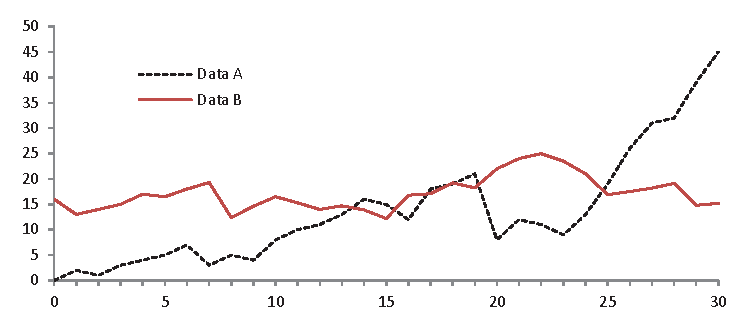
\includegraphics[width=\textwidth]{fig1.eps}
\caption{A figure caption is always placed below the illustration.
Please note that short captions are centered, while long ones are
justified by the macro package automatically.} \label{fig1}
\end{figure}

Program listings or code snippets in the text like \lstinline!var i:integer;!
should be set in typewriter font. The ``listings'' macro package can be used
for reader-friendly syntax highlighting as in the following Pascal sample code:\footnote{For
typesetting pseudocode, the ``algorithmic'', ``algorithm2e'', ``algorithmicx'',
and ``program'' packages are also worth considering.}
\begin{lstlisting}
for i:=maxint to 0 do
begin
    { do nothing }
end;
Write('end of sample code');
\end{lstlisting}


\begin{theorem}
This is a sample theorem. The run-in heading is set in bold, while
the following text appears in italics. Definitions, lemmas,
propositions, and corollaries are styled the same way.
\end{theorem}
%
% the environments 'definition', 'lemma', 'proposition', 'corollary',
% 'remark', and 'example' are defined in the LLNCS documentclass as well.
%
\begin{proof}
Proofs, examples, and remarks have the initial word in italics,
while the following text appears in normal font.
\end{proof}
For citations of references, we prefer the use of square brackets
and consecutive numbers. Citations using labels or the author/year
convention are also acceptable. The following bibliography provides
a sample reference list with entries for journal
articles~\cite{ref_article1}, an LNCS chapter~\cite{ref_lncs1}, a
book~\cite{ref_book1}, proceedings without editors~\cite{ref_proc1},
and a homepage~\cite{ref_url1}. Multiple citations are grouped
\cite{ref_article1,ref_lncs1,ref_book1},
\cite{ref_article1,ref_book1,ref_proc1,ref_url1}.

\subsubsection{Acknowledgements} Please place your acknowledgments at
the end of the paper, preceded by an unnumbered run-in heading (i.e.
3rd-level heading).


%
% ---- Bibliography ----
%
% BibTeX users should specify bibliography style 'splncs04'.
% References will then be sorted and formatted in the correct style.
%
% \bibliographystyle{splncs04}
% \bibliography{mybibliography}
%
\begin{thebibliography}{8}
\bibitem{ref_article1}
Author, F.: Article title. Journal \textbf{2}(5), 99--110 (2016)

\bibitem{ref_lncs1}
Author, F., Author, S.: Title of a proceedings paper. In: Editor,
F., Editor, S. (eds.) CONFERENCE 2016, LNCS, vol. 9999, pp. 1--13.
Springer, Heidelberg (2016). \doi{10.10007/123456789_0}

\bibitem{ref_book1}
Author, F., Author, S., Author, T.: Book title. 2nd edn. Publisher,
Location (1999)

\bibitem{ref_proc1}
Author, A.-B.: Contribution title. In: 9th International Proceedings
on Proceedings, pp. 1--2. Publisher, Location (2010)

\bibitem{ref_url1}
LNCS Homepage, \url{http://www.springer.com/lncs}. Last accessed 4
Oct 2017
\end{thebibliography}
\end{document}
